\section{Intervalle critique dans la bifurcation de fold}
Soit l'EDO à 1 paramètre
\begin{equation}
  \dot{x}(t) = a_1x^3 + a_2x + \phi \equiv f_{\phi}(x), \quad a_1, a_2 \in \R
\end{equation}
On peut la voir comme la somme d'une fonction cubique et d'une droite. En traçant les 2 graphes, on observe que l'on a plusieurs équilibres pour $a_1 < 0 < a_2$ ou $a_2 < 0 < a_1$. Il existe au moins un équilibre lorsque la droite et la fonction cubique s'intersectent.
\begin{equation} \label{eq:intersection}
  f_{\phi_c}(x_0) = 0 \iff a_1 x_0^3 = - (a_2x_0 + \phi_c)
\end{equation}
Il y a création de 3 équilibres lorsque la droite est tangente à la fonction cubique.
\begin{align*}
  f'_{\phi_c}(x_0) = 0
    &\iff 3a_1 x_0^2 = -a_2 \\
    &\iff x_0^2 = - \frac{a_2}{3a_1} \\
    &\iff x_0 = \pm \sqrt{- \frac{a_2}{3a_1}}
\end{align*}
ce qui implique en injectant dans (\ref{eq:intersection}) que
\begin{align*}
  \pm a_1 \left( - \frac{a_2}{3a_1} \right)^{3/2}
    &= - \left( \pm a_2 \left[ - \frac{a_2}{3a_1} \right]^{1/2} + \phi_c \right) \\
  \iff \phi_c
    &= \mp a_1 \left( - \frac{a_2}{3a_1} \right)^{3/2} \mp a_2 \left( - \frac{a_2}{3a_1} \right)^{1/2} \\
    &= \mp a_1 \left( - \frac{a_2}{3a_1} \right)^{3/2} \mp a_2 \left( - \frac{a_2}{3a_1} \right)^{1/2} \frac{3}{3} \\
    &= \pm \frac{4(-a_2)^{3/2}}{(27a_1)^{1/2}}
\end{align*}

On a donc trouvé l'intervalle critique où il y a création de 3 équilibres.
\begin{equation}
  |\phi_c| < \sqrt{\frac{-4(a_2)^3}{27a_1}}
\end{equation}
pour $a_1 < 0 < a_2$ ou $a_2 < 0 < a_1$.

% \section{La bifurcation de Hopf a un unique équilibre en $(y,z)=(0,0)$}
% Soit le système d'EDO,
% \begin{equation}
%   \begin{cases}
%     \dot{y} = b_1z + b_2[\gamma - (y^2 + z^2)]y \equiv f_{1,\gamma}(y,z) \\
%     \dot{z} = c_1y + c_2[\gamma - (y^2 + z^2)]z \equiv f_{2,\gamma}(y,z)
%   \end{cases}
% \end{equation}
% avec $b_1, b_2, c_1, c_2 \in \R_{\ast}$.

% Il y a équilibre lorsque $\vb{f}_{\gamma}(y,z) = 0$ c'est à dire,
% \begin{align*}
%   \vb{f}_{\gamma}(y,z) = 0
%     &\iff
%   \begin{cases}
%     0 &= b_1z + b_2[\gamma - (y^2 + z^2)]y \\
%     0 &= c_1y + c_2[\gamma - (y^2 + z^2)]z
%   \end{cases} \\
%     &\implies
%   \begin{cases}
%     b_1z &= b_2[\gamma - (y^2 + z^2)]y \\
%     0 &= c_1y + c_2[\gamma - (y^2 + z^2)]^2 \frac{b_2}{b_1} y
%   \end{cases}
% \end{align*}

% On trouve donc,
% \begin{equation*}
%   0 = y \left( c_1 - c_2 \frac{b_2}{b_1} \underbrace{[\gamma - (y^2 + z^2)]^2}_{\equiv \eta} \right)
% \end{equation*}

% Ce qui implique que $y = 0$ si $c_1 \neq c_2 \frac{b_2}{b_1}$.

% Si $y = 0$ alors $z = 0$ et $(y,z) = (0,0)$ est le seul équilibre réel de ce système.

\section{Le système secondaire avec paramètre de forçage a un cycle limite}

Sans perte de généralités, posons $b_1 = b_2 = 1$ et $c_1 = -1$ et $c_2 = 1$.

Le système (\ref{eq:hopf}) devient,
\begin{equation}
  \begin{cases}
    \dot{y} &= 1z + 1[\gamma - (y^2 + z^2)]y \\
    \dot{z} &= -1y + 1[\gamma - (y^2 + z^2)]z
  \end{cases}
\end{equation}
Passons en coordonnées polaires $(r, \theta)$\footnote{On retrouve facilement les relations de changement de coordonnées en dérivant $r^2 = y^2 + z^2$ et $\theta = \arctan(z/y)$}.
\begin{align*}
  \dot{r} = \frac{y\dot{y} + z\dot{z}}{r}
    &= \frac{y(z + \gamma y - r^2 y) + z(-y + \gamma z - r^2 z)}{r} \\
    &= \frac{\gamma(y^2 + z^2) - r^2(y^2 + z^2)}{r} \\
    &= \frac{\gamma r^2 - r^4}{r} \\
    &= \gamma r - r^3
\end{align*}
\begin{align*}
  \dot{\theta} = \frac{\dot{z}y - z\dot{y}}{r^2}
    &= \frac{(-y + \gamma z - r^2 z)y - z(z + \gamma y - r^2 y)}{r^2} \\
    &= \frac{- y^2 - z^2}{r^2} \\
    &= -1
\end{align*}
L'EDO en $\dot{\theta}$ est facilement résolvable par séparation des variables. On trouve $\theta = -t + \theta_0$. L'analyse graphique de l'équation pour $\dot{r}$ nous renseigne sur la nature des équilibres de cette dernière.
On trouve en effet aisément que cette EDO a des équilibres en $r = 0$ pour tout $\gamma \in \R$ et $r = \sqrt{\gamma}$ pour $\gamma \geq 0$.

L'analyse graphique nous montre que,
\begin{itemize}
  \item pour $\gamma < 0$, l'équilibre en $r = 0$ est un attracteur.
  \item pour $\gamma \geq 0$, l'équilibre en $r = 0$ est une source et $r = \sqrt{\gamma}$ est un attracteur.
\end{itemize}

Cela nous montre bien l'apparition d'un cycle limite dans le plan $(y,z)$ pour des valeurs de $\gamma \geq 0$.

L'équation pour $\dot{\theta}$ nous montre que les trajectoires ont un sens horloger (autour de l'origine) tandis que l'équation paramétrique de ce cycle limite est donnée par,
\begin{equation}
  \begin{cases}
    y &= \sqrt{\gamma} \sin(\theta_0 - t) \\
    z &= \sqrt{\gamma} \cos(\theta_0 - t)
  \end{cases}
\end{equation}

Ci-dessous le portrait de phase du système $(\ref{eq:hopf})$ pour $\gamma = 1$. On voit bien les solutions converger vers ce cycle.
\begin{figure}[H]
  \centering
  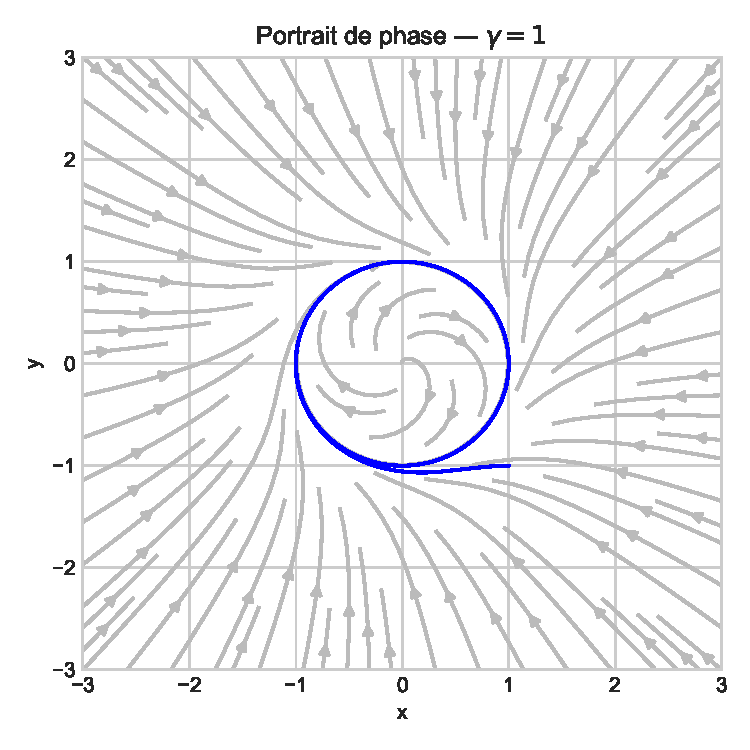
\includegraphics{figures/phase-plot.pdf}
  \caption{Portrait de phase du système d'équations différentielles (\ref{eq:hopf}) pour $\gamma = 1$. Le cycle limite est affiché en bleu.}
  \label{fig:phase-plot}
\end{figure}

\section{Paramètres utilisés dans les simulations}
\begin{table}[H]
\centering
\begin{tabular}{lcc} \toprule
  & \multicolumn {2}{c}{Valeur} \\\cmidrule(lr) {2-3}
  Paramètre         & Non-Stochastique                & Stochastique\\\hline
  $\phi(t)$         & $0.5t$                          & $0.5t$ \\
  $\gamma_1$        & $-0.1$                          & $-0.2$ \\
  $\gamma_2$        & $0.12$                          & $0.3$ \\
  $a_1$             & $-1$                            & $-1$ \\
  $a_2$             & $1$                             & $1$ \\
  $b_1$             & $1$                             & $0.1$ \\
  $b_2$             & $1$                             & $1$ \\
  $c_1$             & $-1$                            & $-0.5$ \\
  $c_2$             & $1$                             & $1$ \\
  $t$               & $[0, 500]$                      & $[0, 500]$ \\
  $\Delta t$        & $0.2$                           & $0.1$ \\
  $(x_0, y_0, z_0)$ & $(-0.5, 1, -1)$                 & $(-0.5, 1, -1)$ \\
  Moyenne           & //                              & $0$ \\
  Variance          & //                              & $0.1$ \\\hline
\end{tabular}
\caption{Au centre, les paramètres utilisés dans les différentes bifurcations et la série temporelle non stochastique. A droite, les paramètres utilisés dans la série temporelle stochastique}
\label{tab:parameters}
\end{table}
